\section{Evaluation of the critical law}\label{sec:experiments}
The experiments assess the two prediction steps separately.
The readout comparison conditions on observed imbalance to isolate internal
variation. The terminal comparison assesses the diffusion and unconditional
overflow mean. All evaluations use preserved samples and frozen lookup tables.
The profile readout has no fitted parameter.

\subsection{Certified evaluation}\label{sec:numerics}
The profile has no closed form here. An a posteriori certificate evaluates it from
a saved probability trajectory, with binary64 inputs treated as exact rationals.
It combines a full polynomial residual, analytic infinite-tail bounds, and
lower transition kernels for the midpoint difference equation.
The uniform profile error is $D_*<9.038\,10^{-6}$.
The resulting certified interval
\[
 S_0(0)\in[0.63127654,\,0.63129462]
\]
shows the size of the internal contribution even at zero imbalance.
The restoring coefficient satisfies
$-\gb'(0)\in[0.71997987,\,0.72012468]$.
Supplement sections~\ref*{app:tails} and~\ref*{app:certificate} give the
construction, failed early stages, and all reported readout bounds.
These are deterministic bounds on the limiting profile, not finite-$q$ error bars.

Figure~\ref{fig:mechanism} shows the two-side profile and averaged response
from the saved numerical nodes. The different side laws record the tie rule.
Their half-phase shift agrees with the identity proved in
Section~\ref{sec:profile}. The response points toward zero imbalance and
saturates at large imbalance, as required by Theorem~\ref{thm:limit}.


\subsection{The internal contribution at observed imbalance}\label{sec:ablation}
For each saved endpoint at $n_*=q^2$ and $\kappa=1$, compare
\[
 x=Z_c(n_*)/q,\qquad b=|\Delta_{n_*}|/(2q),\qquad
 p=S_0(\Delta_{n_*}/q).
\]
Figure~\ref{fig:profileablation} compares the two readouts at the same observed
imbalance. Across all four cells, mean absolute error falls from
$0.3961$--$0.4355$ to $0.0174$--$0.0180$, a $95.6$--$95.9\%$ reduction.
These are descriptive summaries against a mechanistic simplification.
The configuration audit and duplicate-label treatment are in Supplement
section~\ref*{app:artifact}.

\subsection{Finite-scale errors}
The original batch uses $q=64,128,256,512$, $\lambda=0,1,2$, and matching or
product crosses. It has respectively 128, 128, 256, and 1024 labels per cell.
Feedback error compares the actual conditional cross response with
$g(h_n,\Delta_n/q)$ at 16 prescribed phases.
Overflow error is the maximum of $|Z_c/q-S_h(\Delta/q)|$ over the five
prescribed offsets $h=-1,-1/2,0,1/2,1$.
Figure~\ref{fig:finite} summarizes the nonzero-coupling cells descriptively.
The two errors concern different steps of the proof; neither is a direct
estimate of distance to the limiting path law.

At $q=512$, the frozen inference supports population failure probability
at most $0.10$ for feedback margin $0.10$ and overflow margin $0.05$.
Overflow failures remain, with probability upper bounds $0.058$--$0.073$.
The original cross-kernel CDF bounds are at most $0.130602$.
Supplement section~\ref*{app:original} gives every primary cell and the
separate joint error allocation of at most $0.05$.

\begin{figure}[t]
\centering
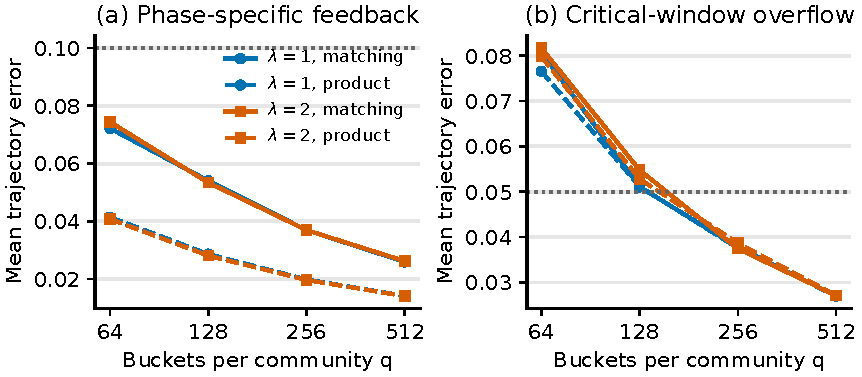
\includegraphics[width=\textwidth]{figures/finite_scale.pdf}
\caption{Descriptive finite-scale errors from the original saved outcomes.
Left: mean per-trajectory feedback RMS over 16 phases.
Right: mean per-trajectory maximum overflow error over five offsets.
Line styles distinguish matching and product kernels; markers distinguish
$\lambda=1,2$. The horizontal lines show the frozen per-trajectory margins,
not confidence limits for these plotted means. Shared labels are not pooled.
No convergence rate is fitted.}
\label{fig:finite}
\end{figure}

\subsection{Terminal diffusion and unconditional overflow}\label{sec:endtoend}
A separately frozen prospective batch has $q=512$, $\kappa=1$,
$\lambda=1,2$, and matching or product crosses. Its four cells each have
4096 labels. The labels are shared across cells, giving 16384 endpoints
rather than 16384 independent observations.
The targets are the unconditional mean difference
$\E[Z_c(q^2)/q]-\E[S_0(D_1)]$ and the Kolmogorov distance between
$\cL(\Delta_{q^2}/q)$ and $\cL(D_1)$.
The reference uses 32768 preserved SDE paths per $\lambda$, with 16384 Euler
steps per path. No observed microscopic imbalance enters its overflow mean.

\begin{figure}[t]
\centering
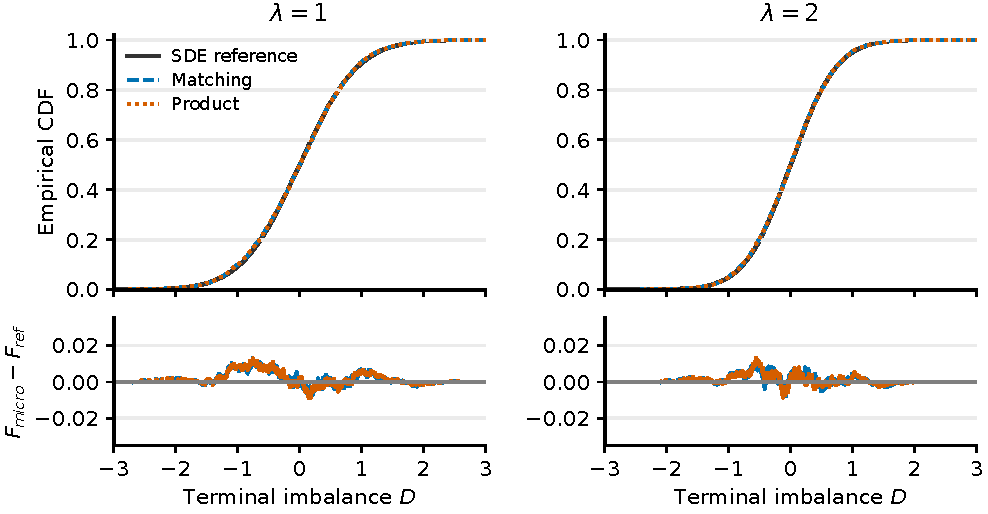
\includegraphics[width=\textwidth]{figures/terminal_law.pdf}
\caption{Terminal imbalance: the two prospective microscopic empirical CDFs
and the independently generated, preserved SDE reference for each $\lambda$.
The lower panels show microscopic minus reference empirical CDFs at all jumps.
Each microscopic cell has 4096 labels; each reference has 32768 paths.
The curves are descriptive; the numerical and sampling allowances enter the
distance bounds in Table~\ref{tab:prospective}.}
\label{fig:terminal}
\end{figure}

\begin{table}[t]
\caption{Prospective comparisons at $q=512$, $\kappa=1$.
Mean intervals bound microscopic mean overflow minus the SDE mean readout.
CDF upper bounds concern terminal imbalance and have lower bound zero.
All displayed limits are rounded outwards and include reference error.}
\label{tab:prospective}
\centering\small
\begin{tabular}{clcc}\toprule
$\lambda$ & Cross kernel & Mean-difference interval & CDF upper bound\\\midrule
1 & matching & $[-0.00840,\ 0.01010]$ & 0.06542\\
1 & product  & $[-0.00860,\ 0.00993]$ & 0.06500\\
2 & matching & $[-0.00663,\ 0.00844]$ & 0.07021\\
2 & product  & $[-0.00671,\ 0.00834]$ & 0.07119\\\bottomrule
\end{tabular}
\end{table}

All mean intervals lie within the frozen $[-0.05,0.05]$ margin.
All CDF upper bounds lie below the frozen $0.20$ margin.
The eight comparisons have joint failure allocation below $0.018138367441$,
giving at least $95\%$ coverage under the ideal input-word and reference-arithmetic
contracts in Supplement sections~\ref*{app:inference} and~\ref*{app:sdebudget}.
Coverage is unconditional over the reused reference and fresh data, in a separate
family from the original claims. It requires independent words across labels and
fresh streams independent of prior history. Pseudorandom reproducibility does
not prove these premises. The old reference has no saved register snapshot.

The two comparisons answer different questions. The readout comparison
isolates internal variation at an observed imbalance. The prospective comparison
assesses the predicted imbalance law and unconditional overflow mean.
Together they support the model's interpretation at the tested parameters;
they do not establish a finite-size rate or validation for every fixed kernel.
